\subsection{Correnti di polarizzazione}

In questa parte dell'esperienza abbiamo progettato diversi circuiti per misurare la corrente di polarizzazione per entrambi gli ingressi, avendo già stabilizzato la tensione di offset dall'esterno. Di seguito proponiamo due modalità.

\subsubsection{Configurazione senza retroazione}

\begin{wrapfigure}[16]{r}{0.55\textwidth}
  \begin{center}
    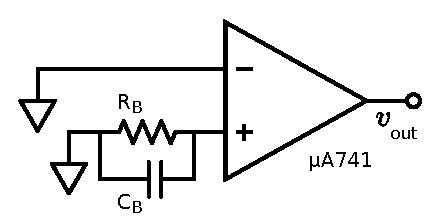
\includegraphics[width=0.30\textwidth]{../E02/latex/direct_measure.pdf}
  \end{center}
  \caption{Schema del circuito non retro-azionato utilizzato per stimare la corrente di polarizzazione. La resistenza utilizzata è $R_B=10.36\pm0.01$\si{\mega\ohm}; la capacità $C_B=102 \pm 1$ \si{\nano\farad}.}
  \label{circuito:rel2_correnti_senzaretroazione}
\end{wrapfigure}

Nel circuito mostrato in figura abbiamo posto la resistenza all'ingresso non invertente (analogamente si può fare con l'ingresso invertente) e, misurando la caduta di potenziale ai capi della stessa con il multimetro, possiamo ottenere il valore di corrente desiderato applicando semplicemente la legge di Ohm

$$V=I_{b^+} R$$

Per far ciò, dato che attendevamo una corrente dell'ordine dei \si{\nano\ampere}, abbiamo utilizzato una resistenza molto grande in modo da poter leggere il valore della tensione su una scala accettabile per il multimetro.

Durante la procedura abbiamo però notato che, a causa di rumori ambientali, il valore di tensione sul multimetro fluttuava sulla prima cifra, rendendo nostra misurazione ovviamente non quantitativa (al massimo poteva stimarci l'ordine di grandezza della corrente). Per ovviare, abbiamo inserito in parallelo alla resistenza un condensatore che caricandosi si portava alla stessa ddp dei capi della resistenza. In questo modo abbiamo potuto ottenere un valore meno fluttuante, che si attestava a $V=(-80 \pm 2)$ \si{\milli\volt}, cioè $I_{b^+}=(7.7 \pm 0.2)$ \si{\nano\ampere}.

Con questo metodo semplice abbiamo potuto ottenere una prima stima del valore della corrente. Di contro bisogno considerare che il rumore non permette di avere una stima qualitativa ed inoltre la resistenza, scaldandosi, modifica il suo valore e potrebbe portare ad un errore sulla misura. Nel paragrafo successivo progetteremo dunque un circuito che, sfruttando l'amplificazione data dall'amplificatore operazionale, minimizzerà questi errori.

\subsubsection{Configurazione con retroazione negativa}

Sfruttando un modello simile a quello utilizzato per trovare la tensione di offset, abbiamo montato i circuiti come in figura. Data la tensione in uscita, grazie alle proprietà di amplificazione dei segnali in ingresso dell'OPAMP, possiamo ottenere una misura indiretta della corrente di polarizzazione.

\paragraph{Misura di $I_{b^-}$}

\begin{wrapfigure}[15]{l}{0.55\textwidth}
  \begin{center}
    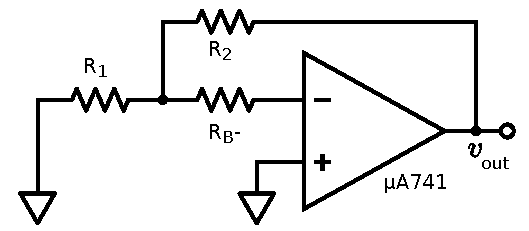
\includegraphics[width=0.30\textwidth]{../E02/latex/inv_current.pdf}
  \end{center}
  \caption{Schema del circuito retro-azionato utilizzato per stimare la corrente di polarizzazione $I_{b^-}$. Le resistenze utilizzate sono $R_1=100\pm1$\si{\ohm}, $R_2=99.8\pm0.1$\si{\kilo\ohm} e $R_B=99.9\pm0.1$\si{\kilo\ohm}.}
  \label{circuito:rel2_correnti_retroazione_inv}
\end{wrapfigure}

Risolviamo il circuito per trovare la corrente di polarizzazione $I_{b^-}$ in funzione della tensione di uscita. Considerando $V_{-}$ la tensione al capo di $R_B$ collegato all'OPAMP e $V^*$ quello opposto, vale in quel punto la legge di Kirchhoff sui nodi

$$\frac{V^* - V_{in}}{R_1} + \frac{V^*-V_{out}}{R_2} + \frac{V^*-V_{-}}{R_B}=0$$

Dato che l'amplificatore operazionale è considerato già stabilizzato per quanto riguarda la tensione di offset, possiamo considerare la tensione all'ingresso invertente uguale all'ingresso non invertente. Vale dunque che $V_{in}=V_{-}=0$ e si trova (considerando $I_{b^-} R_B = V^*$):

$$I_{b^-}=\frac{V_{out}}{R_2 R_B}\frac{1}{\frac{1}{R_1}+\frac{1}{R_2}+\frac{1}{R_B}}$$

Le resistenze sono state dimensionate tenendo invece conto dell'ordine di grandezza della corrente da misurare e considerando il risultato sopra ottenuto: volevamo che $V_{out}$ fosse almeno $10^7\approx10^8$ volte più grande della corrente, per poter utilizzare il multimetro, che ha scale di misura limitate. I valori sono in Figura \ref{circuito:rel2_correnti_retroazione_inv}.

La misura di tensione di uscita è di $370.3$ \si{\milli\volt} ed il valore ottenuto è dunque $I_{b^-} = (3.7 \pm 0.1)$ \si{\nano\ampere}.

\paragraph{Misura di $I_{b^+}$}

\begin{wrapfigure}[15]{r}{0.55\textwidth}
  \begin{center}
    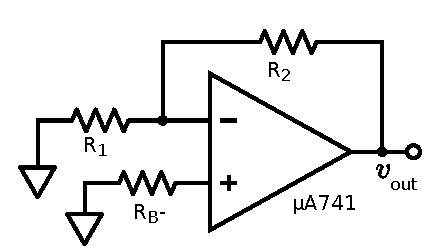
\includegraphics[width=0.25\textwidth]{../E02/latex/ninv_current.pdf}
  \end{center}
  \caption{Schema del circuito retro-azionato utilizzato per stimare la corrente di polarizzazione $I_{b^+}$. Le resistenze utilizzate sono le medesime del circuito precedente: $R_1=100\pm1$\si{\ohm}, $R_2=99.8\pm0.1$\si{\kilo\ohm} e $R_B=99.9\pm0.1$\si{\kilo\ohm}.}
  \label{circuito:rel2_correnti_retroazione_noninv}
\end{wrapfigure}

Similmente a quanto visto per la configurazione prima, troviamo che, data la legge di Kirchhoff (con $V^*$ la tensione all'ingresso non invertente, che per quanto detto sopra è uguale a quella all'ingresso invertente)

$$\frac{V^* - V_{in}}{R_1} + \frac{V^*-V_{out}}{R_2}=0$$

e considerando $V^*=I_{b^+} R_B$, otteniamo

\begin{equation}
I_{b^+}=\frac{V_{out}}{R_2 R_B}\frac{1}{\frac{1}{R_1}+\frac{1}{R_2}}
\label{eq2:corrente_noninv}
\end{equation}

Anche in questo caso le resistenze sono state dimensionate come sopra e i valori sono in Figura \ref{circuito:rel2_correnti_retroazione_noninv}. La misura di tensione di uscita è di $-362.7$ \si{\milli\volt} ed il valore ottenuto è dunque $I_{b^+} = - (3.6 \pm 0.1)$ \si{\nano\ampere} \footnote{La negatività della corrente va intesa rispetto all'ingresso non invertente, ed è quindi uscente rispetto a tale ingresso. Al contrario, nel paragrafo precedente, la corrente è intesa entrante nel punto di $V^*$, e quindi è entrante rispetto all'ingresso invertente.}.

\paragraph{Calcolo di $I_{b^+}$ data $I_{b^-}$}

Consideriamo ora un altro modo per trovare la corrente di polarizzazione $I_{b^+}$ supponendo di aver già effettuato la misura di $I_{b^-}$ nel primo circuito (Figura \ref{circuito:rel2_correnti_retroazione_inv}). Successivamente controlleremo che il valore 'sperimentale' calcolato con (\ref{eq2:corrente_noninv}) è compatibile con quello calcolato in questo paragrafo.

Analizziamo dunque il secondo circuito (Figura \ref{circuito:rel2_correnti_retroazione_noninv}) per cercare di trovare la dipendenza di $I_{b^+}$ da $I_{b^-}$. Vale, dalla teoria

$$V_{out} = \left( 1+\frac{R_2}{R_1} \right)\left[ \frac{I_{b^-}R_2}{\frac{R_1+R_2}{R_1}} - I_{b^+} R_B\right]$$

da cui è possibile ricavare

$$I_{b^+} = \frac{R_1}{R_B(R_1+R_2)}(I_{b^-}-V_{out})$$

ed inserendo i valori otteniamo $I_{b^+} = - (3.6 \pm 0.1)$ \si{\nano\ampere}, compatibile con il risultato precedente.